\documentclass[11pt,a4paper]{article}

\usepackage[margin=0.95in,top=1.05in,bottom=1.05in]{geometry}
\usepackage{amsmath,amssymb,mathtools}
\usepackage{booktabs,array}
\usepackage{graphicx}
\usepackage{xcolor}
\usepackage{xeCJK}
\usepackage[most]{tcolorbox}
\usepackage{fancyhdr}
\usepackage{titlesec}
\usepackage{hyperref}

\setCJKmainfont[BoldFont={NanumMyeongjoExtraBold}]{Nanum Myeongjo}
\setCJKsansfont{Apple SD Gothic Neo}
\linespread{1.26}
\setlength{\parskip}{0.36em}
\setlength{\parindent}{0pt}
\renewcommand{\figurename}{\sffamily\bfseries 그림}
\renewcommand{\tablename}{\sffamily\bfseries 표}

\definecolor{navy}{HTML}{0F172A}
\definecolor{royal}{HTML}{1D4ED8}
\definecolor{teal}{HTML}{0D9488}
\definecolor{rose}{HTML}{E11D48}
\definecolor{amber}{HTML}{B45309}
\definecolor{softbg}{HTML}{F8FAFC}
\definecolor{softteal}{HTML}{F0FDFA}
\definecolor{softamber}{HTML}{FFFBEB}

\hypersetup{
  colorlinks=true,
  linkcolor=royal,
  urlcolor=royal,
  pdftitle={다각형이 들을 수 없는 파동들: 소련 우파(Ufa)의 잊힌 수학에서 발굴한 7가지 기적}
}

\titleformat{\section}
  {\sffamily\Large\bfseries\color{navy}}
  {\textcolor{teal}{\thesection.}}{0.6em}{}
  [\vspace{2pt}\titlerule]

\titleformat{\subsection}
  {\sffamily\large\bfseries\color{royal}}
  {\thesubsection}{0.4em}{}

\pagestyle{fancy}
\fancyhf{}
\fancyhead[L]{\sffamily\footnotesize\color{gray} Project ReMath · 수학 고고학 특집 해설}
\fancyhead[R]{\sffamily\footnotesize\color{gray} 다각형이 들을 수 없는 파동들 (A.~F.~Leont'ev 발굴 프로젝트)}
\fancyfoot[C]{\sffamily\small\thepage}
\renewcommand{\headrulewidth}{0.4pt}

\newtcolorbox{wowbox}[1]{
  enhanced,
  colback=softteal,
  colframe=teal,
  boxrule=0.9pt,
  arc=3pt,
  left=10pt,right=10pt,top=7pt,bottom=7pt,
  fonttitle=\sffamily\bfseries,
  title={#1}
}

\newtcolorbox{storybox}[1]{
  enhanced,
  colback=softamber,
  colframe=amber,
  boxrule=0.9pt,
  arc=3pt,
  left=10pt,right=10pt,top=7pt,bottom=7pt,
  fonttitle=\sffamily\bfseries,
  title={#1}
}

\begin{document}

\begin{center}
  {\sffamily\footnotesize\bfseries\color{teal} MATHEMATICAL ARCHAEOLOGY · 수학 고고학 리포트}\\[0.55em]
  {\sffamily\huge\bfseries\color{navy} 다각형이 들을 수 없는 파동들}\\[0.4em]
  {\sffamily\large\color{darkgray} 소련 우파(Ufa)의 잊힌 지수급수 이론에서 발굴한 7가지 수학적 기적}\\[0.9em]
  {\sffamily\small Project ReMath \quad|\quad 2026년 11월 23일}\\[0.25em]
  {\footnotesize\color{gray} 원전 아카이브: A.~F.~Leont'ev (1969–1987, Math-Net.Ru) · 기계 검증: Lean~4.36.0 (핵심 대수·미니맥스 31개 정리, \texttt{sorry} 0개)}
\end{center}

\vspace{0.4em}

\begin{tcolorbox}[colback=softbg,colframe=navy,boxrule=0.7pt,arc=3pt,left=12pt,right=12pt,top=8pt,bottom=8pt]
\textbf{\sffamily 발굴된 7가지 수학적 기적 한눈에 보기}\\[0.25em]
1970년대 소련 바시키르의 도시 \textbf{우파(Ufa)}에서 수학자 \textbf{알렉세이 레온티예프(A.~F.~Leont'ev)}가 구축했지만 영문 번역본조차 없이 잊혔던 《지수급수(\textit{Ryady eksponent}, 1976)》 이론을 서구의 현대 편미분방정식 해법(\textbf{포카스 통합 변환법})과 정면으로 연결했다. 그 과정에서 모습을 드러낸 7가지 핵심 발견은 다음과 같다:
\textbf{[기적 1]} 동서양 두 스펙트럼 이론의 정확한 잔여 변환과, 정사각형 바깥에서 $10^{27}$로 폭주하면서도 합치면 $0$이 되는 \textbf{유령 파동} ·
\textbf{[기적 2]} 오직 평행사변형에서만 투명한 \textbf{생브낭 탄성 비틀림 응력} 대 정삼각형의 유일한 투명 경계장을 만드는 \textbf{`Y자 리만 제타 해골'} ·
\textbf{[기적 3]} 꼭짓점이 $0.0001$ 라디안만 비틀려도 양방향 투명 모드가 전멸하는 \textbf{대칭 붕괴} ·
\textbf{[기적 4]} 짝수 다각형의 \textbf{홀짝 은폐 역설}과 단일 이동 주파수 해독 ·
\textbf{[기적 5]} 한 도형 안에서 꼭짓점 내각에 따라 수렴 지수가 갈라지는 \textbf{$60^\circ/120^\circ$ 마름모의 두 기울기($N^{-5/6}$ 대 $N^{-2/3}$)} ·
\textbf{[기적 6]} 고정밀 구간연산으로 증명한 \textbf{`반스텝($\theta=1/2$) 최적 신화'의 붕괴} ·
\textbf{[기적 7]} 약 \textbf{24자릿수(23.5 orders) 초해상도 윈도우}, 포카스 PDE 영공간 완치, 그리고 가열 금속판의 꼭짓점 열유속 해독.
\end{tcolorbox}

\section{프롤로그: 철의 장막 뒤에 잠들어 있던 `다각형의 지수급수'}

신호나 물리장을 기본 파동들로 분해할 때 가장 익숙한 도구는 \textbf{푸리에 급수} $\sum c_n e^{inx}$다. 하지만 고전 푸리에 급수는 선분이나 주기 격자처럼 병진이동 대칭이 있는 영역에 맞추어 태어났다. 만약 도형이 복소평면 위의 \textbf{정삼각형, 오각형, 혹은 마음대로 찌그러진 볼록 다각형 $D$}라면 어떨까? 비대칭 다각형 위에서는 지수함수들이 서로 직교하지도 않고, 복소 주파수를 어디에 찍어야 할지조차 자명하지 않다.

\begin{storybox}{인물 노트: 농가 13남매 막내에서 우파(Ufa) 학파의 거장으로}
\textbf{알렉세이 표도로비치 레온티예프(A.~F.~Leont'ev, 1917–1987)}는 러시아 농가 13남매 중 막내로 태어나, 제2차 세계대전 당시 고르키 방어 참호를 파며 학업을 이어갔다. 초월수론의 대가 겔폰트(A.~O.~Gelfond)의 제자로 모스크바 스테클로프 연구소까지 올랐던 그는, 1971년 우랄 산맥 서쪽 바시키르의 수도 \textbf{우파(Ufa)}로 내려가 독자적인 복소해석학 학파를 일구었다. 대표작 《지수급수》(1976, Nauka)를 포함한 그의 3부작 단행본은 사후인 1989년 소련 국가상을 받았지만, 지금까지도 영문 번역본이 출간되지 않았다.
\end{storybox}

레온티예프가 찾아낸 해법은 기하학적으로 놀라울 만큼 명쾌했다. 볼록 $p$-각형 $D$의 꼭짓점을 반시계 방향으로 $\gamma_1, \dots, \gamma_p$, 변 벡터를 $d_j = \gamma_{j+1}-\gamma_j$라 할 때, 각 변에 수직인 스펙트럼 반직선(외향 법선의 켤레 방향)을 따라 찍힌 복소 주파수 격자
\begin{equation}
  \Lambda_+ = \left\{ \nu_{jm} = \frac{2\pi i m}{d_j} : 1 \le j \le p,\; m = 1, 2, 3, \dots \right\}
\end{equation}
만으로 다각형 $D$ 내부의 \textbf{모든 정칙함수 $F(z)$를 지수급수 $\sum_{\nu \in \Lambda_+} c_\nu e^{\nu z}$로 내부 콤팩트 집합 위에서 절대 수렴하게 전개할 수 있다!} 물리적으로는 다각형 내부의 어떤 정상상태 조화 온도장($\Delta q = 0$)이나 복소 유체 퍼텐셜이든, \textbf{$p$개 변을 따라 각각 반복되는 1차원 주기 파동 $p$개의 중첩}으로 내부 어디서나 재현된다는 뜻이다.

여기에는 고전 직교기저에는 없는 역설이 숨어 있다. 레온티예프의 연구를 계승·일반화한 로스토프 학파의 코로베이니크(Yu.~F.~Korobeinik, 1981)가 보였듯, 이 정준 지수계열이 $D$ 내부의 모든 정칙함수를 표현하려면 반드시 \textbf{계수가 $0$이 아닌데도 합이 항등적으로 $0$이 되는 `0의 비자명한 전개(유령 파동)'}가 존재해야 한다. 부품들 사이에 정교한 \textbf{여유분(중복성)}이 있어야만 다각형의 구석까지 함수를 잡아낼 수 있는 것이다.

\section{기적 1: 동서양 두 이론의 조우와 `사각형 밖에서도 죽지 않는 유령 파동'}

레온티예프 타계 10년 뒤인 1997년, 아타나시오스 포카스(A.~S.~Fokas, 이후 2002년 케임브리지대 석좌교수 부임)는 다각형 위 편미분방정식을 푸는 \textbf{통합 변환법(Unified Transform Method)}을 도입했다. 놀랍게도 포카스 해법이 복소 스펙트럼 평면에서 적분하는 $p$개의 반직선은, 레온티예프가 주파수 $\nu_{jm}$을 찍었던 \textbf{바로 그 반직선들과 정확히 일치한다.}

우리는 두 이론을 잇는 정확한 잔여 변환 공식을 증명했다. 한 변의 적분값만으로는 이 정준 계수를 구할 수 없지만(상수함수 $F \equiv 1$조차 자기 변 위의 샘플이 전부 $0$이 된다!), $p$개 반직선의 연속 적분을 모두 모으면 레온티예프의 이산 계수 $c_\nu$로 정확히 변환된다(수치적분 오차 $2.24\times 10^{-10}$, 65자리 복원 오차 $1.55\times 10^{-49}$).

\begin{figure}[ht]
\centering
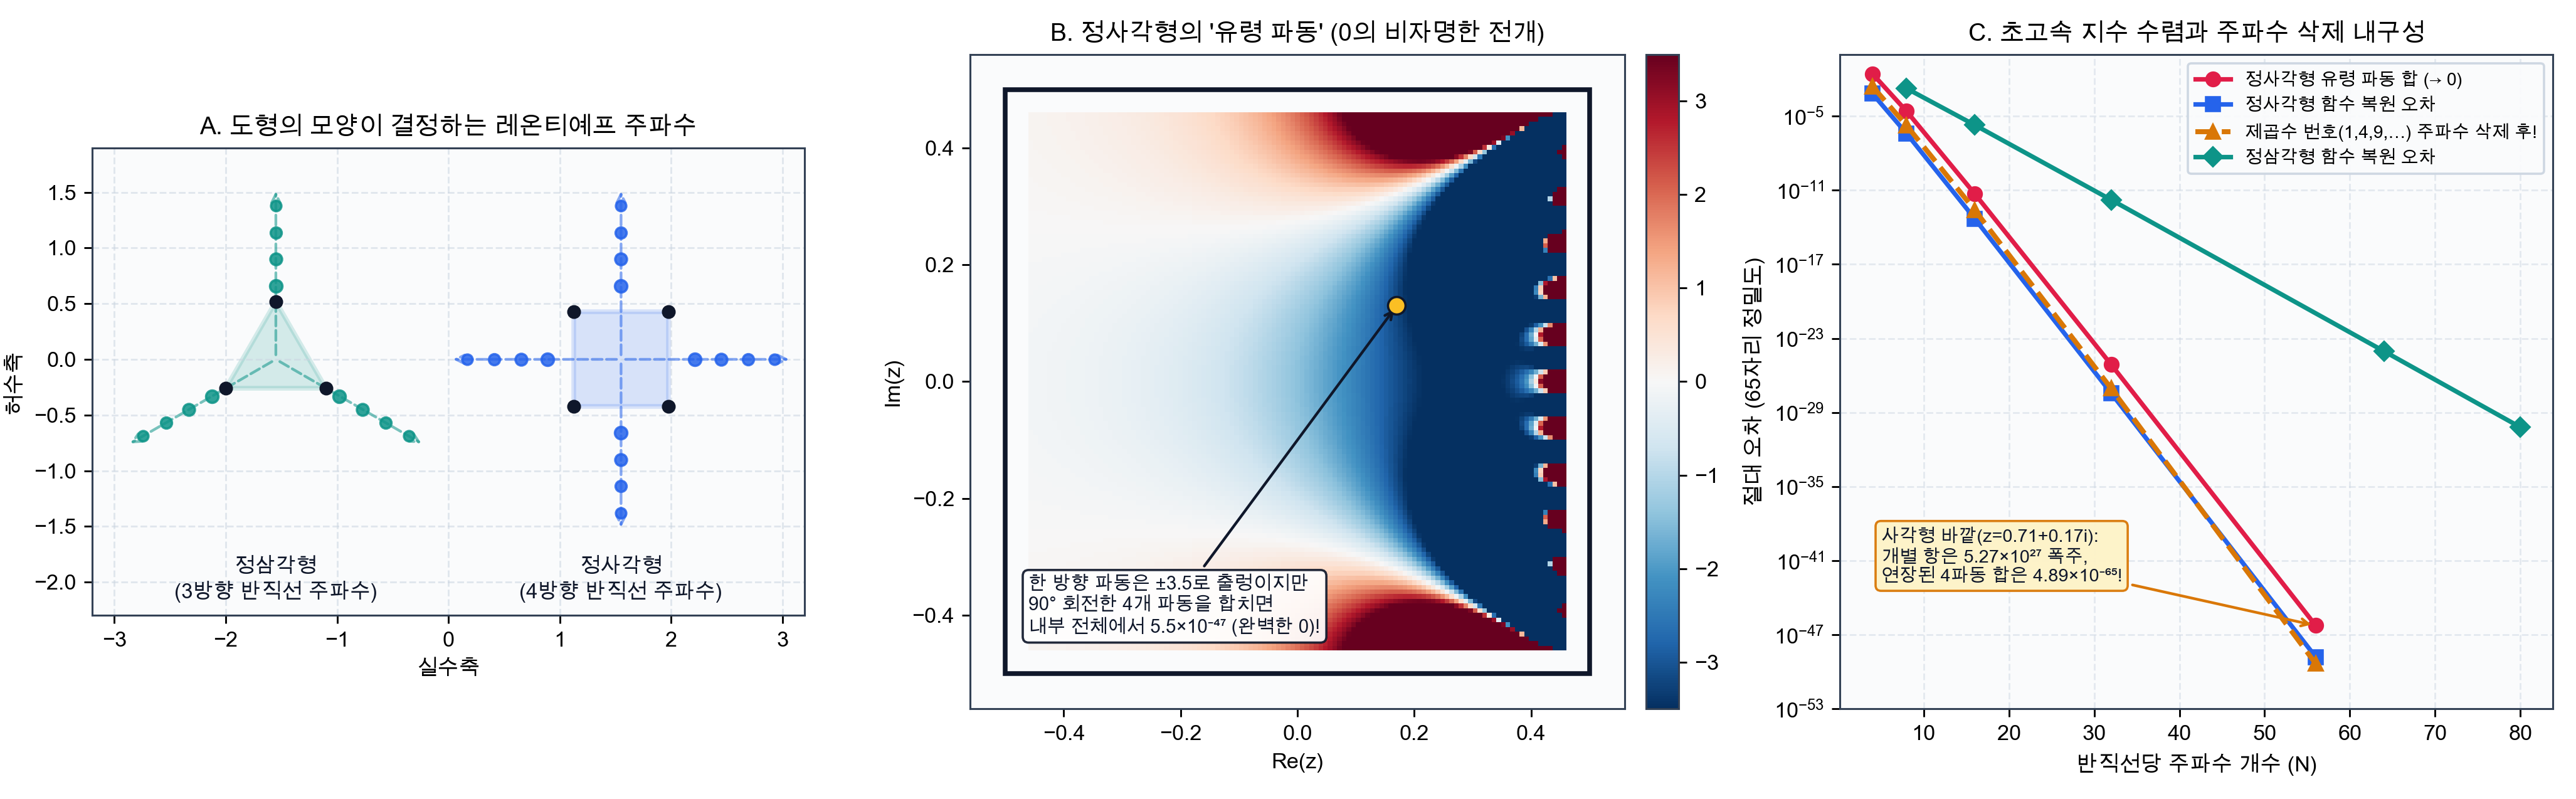
\includegraphics[width=\textwidth]{figs/kr_fig1_concept_and_ghost.png}
\caption{\textbf{A.} 정삼각형(3방향)과 정사각형(4방향)의 기하학이 결정하는 레온티예프 스펙트럼 반직선. \textbf{B.} 정사각형 유령 파동 한 방향 성분의 진동(색상 범위 $\pm 3.5$, $N=12$)과 4방향 합의 상쇄($N=56$에서 $5.5\times 10^{-47}$). \textbf{C.} 제곱수 번호 주파수를 모두 지운 뒤에도 유지되는 지수 수렴.}
\end{figure}

더 극적인 현상은 중심이 원점인 단위 정사각형의 \textbf{유령 파동(Ghost Wave)}에서 나타났다:
\begin{equation}
  G(w) = \sum_{m=1}^\infty \frac{(-1)^m (2\pi m)^2}{2\sinh(\pi m)} e^{2\pi m w}, \qquad
  G(z) + i G(iz) - G(-z) - i G(-iz) \equiv 0.
\end{equation}
\begin{itemize}
  \item 정사각형 내부에서는 각 방향 파동이 거세게 출렁이지만, $90^\circ$ 회전한 네 파동을 더하면 항등적으로 $0$이 된다($z = 0.17+0.13i$, $N=56$ 절단 합에서 \textbf{$5.5\times 10^{-47}$}).
  \item 정사각형 \textbf{바깥}(극점을 피한 $z = 0.71 + 0.17i$)으로 나가면 동쪽 급수의 $m=40$번째 항 하나만 해도 \textbf{$5.27\times 10^{27}$}로 폭주한다. 그런데 이를 람베르트(Lambert) 유리급수로 해석적 연장한 뒤 네 방향을 더하면, 폭주하던 파동들이 맞물려 수치 오차 \textbf{$4.89\times 10^{-65}$}로 완벽히 상쇄된다!
  \item 이 중복성 덕분에 한 변에서 \textbf{모든 제곱수 번호 주파수($m = 1, 4, 9, 16, \dots$)를 지워도} 오차 $4.45\times 10^{-50}$으로 함수가 복원된다(정확한 삭제 한계는 밀도 $0$, 즉 $\#\{\nu \in E : |\nu|\le R\} = o(R)$).
\end{itemize}

\section{기적 2 \& 3: 투명 물리장의 해부와 양방향 대칭 붕괴}

이제 질문을 뒤집어 보자. 다각형 테두리 $\partial D$에 미지의 실수 물리장(전하·열유속) $\mu$가 깔려 있을 때, \textbf{모든 자연 주파수 $\nu \in \Lambda_+$에서 측정값 $B_\mu(\nu) = \int_{\partial D} e^{\nu w}\,d\mu(w)$가 전부 $0$이 되어 절대 감지되지 않는 `투명 물리장'}은 몇 개이며 그 정체는 무엇일까? 임의의 볼록 $p$-각형에 대해 우리가 완성한 분류표는 표~1과 같다.

\begin{table}[ht]
\centering
\caption{임의의 볼록 $p$-각형에서 레온티예프 주파수가 감지하지 못하는 실수 투명 물리장의 정확한 차원.}
\vspace{0.25em}
\small
\begin{tabular}{lrrrr}
\toprule
볼록 $p$-각형 분류 & 단방향 $L^2$ & 단방향 $L^1$ & 단방향 측도 & \textbf{양방향($\Lambda_\pm$) 측도} \\
\midrule
홀수 ($p = 2k+1$: 삼각형, 오각형, $\dots$) & $2k - 1$ & $2k + 1$ & $2k + 1$ & $0$ \\
짝수 ($p = 2k$: 사각형, 육각형, $\dots$) & $2k - 1$ & $2k - 1$ & $2k$ & 중심대칭 $2k$ / 비대칭 $0$ \\
\bottomrule
\end{tabular}
\end{table}

\begin{wowbox}{기적 2-A. 생브낭 탄성 비틀림 응력이 투명한 다각형은 오직 평행사변형뿐이다!}
정사각형($p=4, k=2$)에서 호길이에 대해 제곱적분 가능한($L^2$) 실수 투명 플럭스는 정확히 $3$차원이며, 그 기저는 \textbf{(1) 수평 법선성분 $n_x$}(샘플 잔차 $5.98\times 10^{-67}$), \textbf{(2) 수직 법선성분 $n_y$}, 그리고 대칭 질량-$1$ 대표원인 \textbf{(3) 생브낭(Saint-Venant) 탄성 비틀림 전단응력 $-\partial_n u$} ($-\Delta u = 1,\; u|_{\partial D}=0$, 사각 관 속 푸아죄유 유체 마찰력과 동일)다. 놀랍게도 우리가 증명한 결과, \textbf{균일 생브낭 비틀림 응력이 투명한 볼록 다각형은 오직 평행사변형($p=4$)뿐이다!} 일반 중심대칭 $2k$-각형에서는 균일 밀도가 아니라 $k$개 선분의 확률합인 \textbf{상자-스플라인(box spline)} 밀도의 조화 발레야주가 그 자리를 대신하며, 정삼각형에서는 균일 비틀림이 첫 주파수($m=1$)에서 곧바로 $-0.02203 \ne 0$으로 들통난다.
\end{wowbox}

\begin{figure}[ht]
\centering
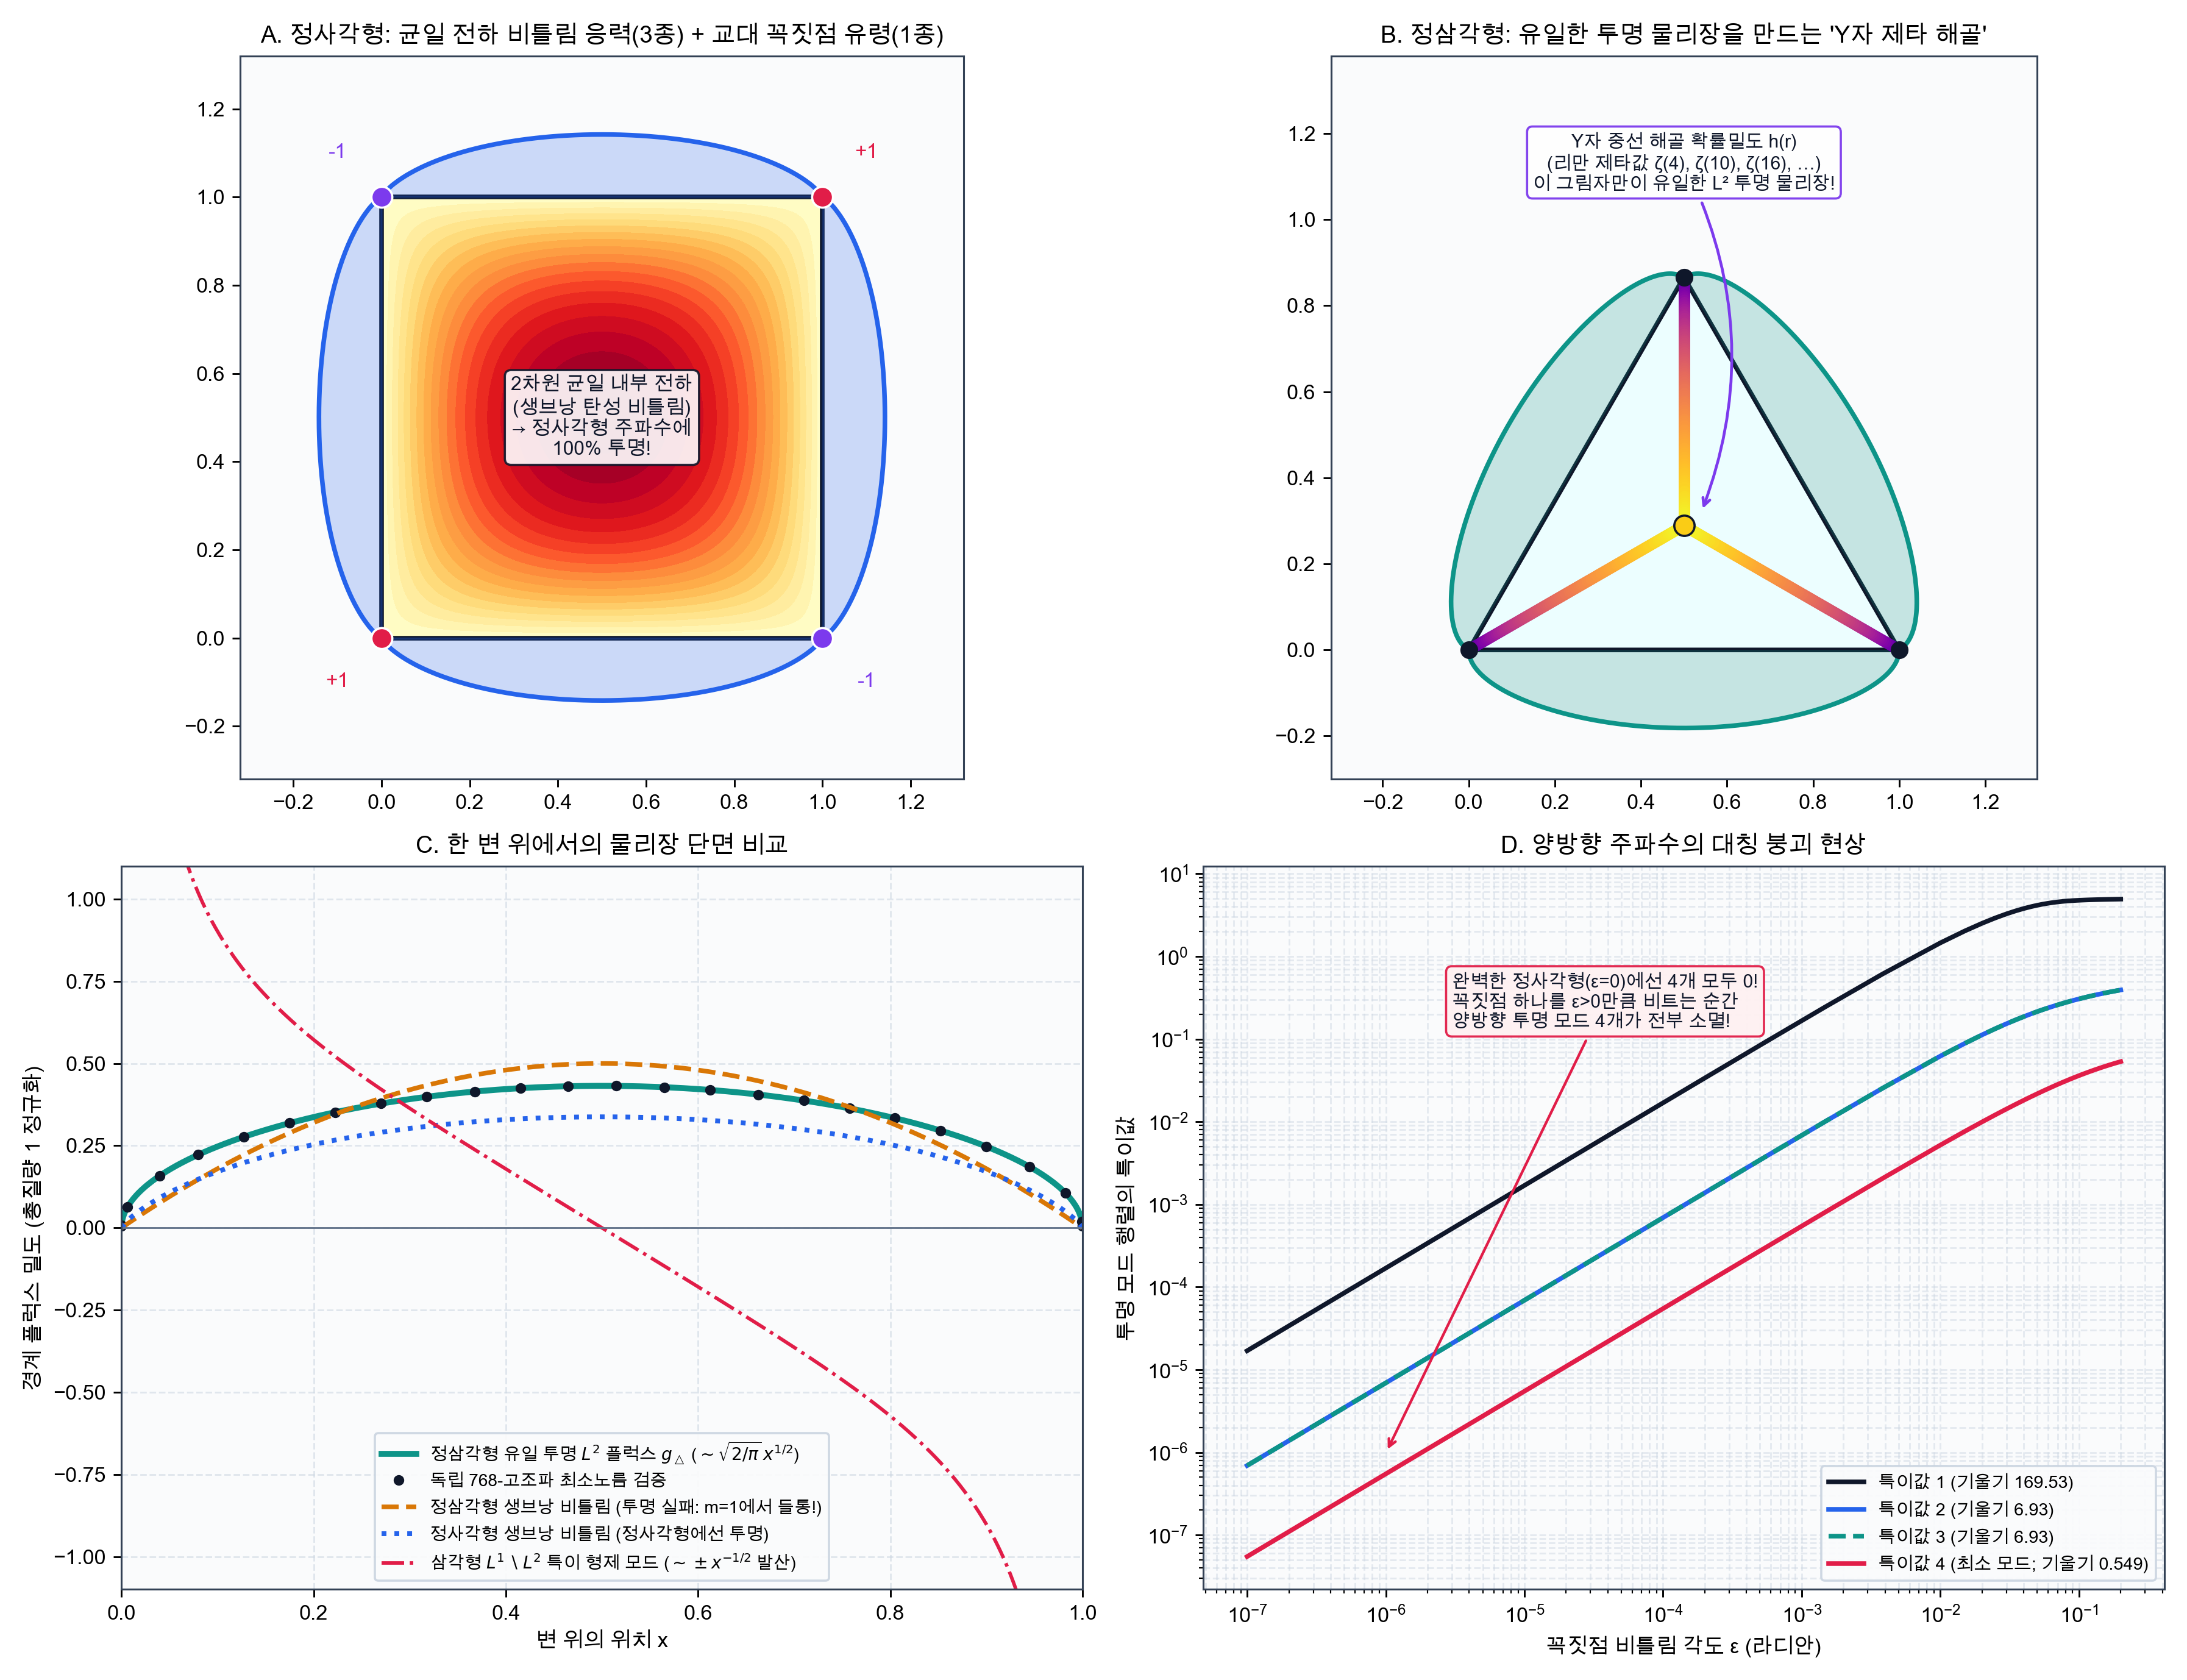
\includegraphics[width=0.95\textwidth]{figs/kr_fig2_square_vs_triangle.png}
\caption{\textbf{A.} 정사각형의 비틀림 응력과 교대 꼭짓점 유령. \textbf{B.} 정삼각형의 유일한 투명 $L^2$ 경계장을 만드는 `Y자 제타 해골' 확률측도와 그림자 $g_\triangle$. \textbf{C.} 질량 정규화된 변 단면 비교 및 $x^{-1/2}$로 발산하는 질량-$0$ 형제 모드. \textbf{D.} 정사각형 꼭짓점을 각도 $\varepsilon$만큼 비틀 때 양방향 투명 모드 4개가 동시에 소멸하는 현상.}
\end{figure}

\begin{wowbox}{기적 2-B. 정삼각형의 유일한 투명 경계장은 `Y자 리만 제타 해골'이 드리운 그림자다!}
정삼각형에 딱 $1$차원 존재하는 총질량 $1$의 유일한 투명 $L^2$ 경계 플럭스 $g_\triangle$를 해부한 결과, 그것은 2차원 면적이 아니라 \textbf{세 꼭짓점과 무게중심을 잇는 3가닥 `Y자 중선 해골' 위에 놓인 양($+$)의 1차원 확률측도}가 세 벽에 드리운 포아송 그림자였다! Binet 감마 공식과 Phragm\'en--Lindel\"of 정리로 증명한 그 반지름 밀도 $h(r) = \sqrt{r}\sum_{n=0}^\infty \frac{e_{3n}}{\Gamma(3n+3/2)} r^{3n}$의 생성함수는 \textbf{리만 제타값 $\zeta(4), \zeta(10), \zeta(16), \dots$}으로 결정되며($e_3 = 6\zeta(4)/\pi$), 꼭짓점 거리 $x \to 0$에서 정확히 $g_\triangle(x) = \sqrt{2/\pi}\,x^{1/2} + O(x^2)$를 따른다(외부 코시 적분 잔차 $3.8\times 10^{-50}$). 또한 정삼각형에는 꼭짓점 양옆에서 $x^{-1/2}$로 발산해 $L^1$에는 속하지만 $L^2$에서 탈락하는 형제 모드 2개가 함께 존재한다.
\end{wowbox}

\textbf{[기적 3: 양방향 대칭 붕괴]} 주파수를 음·양 양방향($\Lambda_\pm$)으로 측정하면 중심대칭 $2k$-각형에서는 $2k$개의 투명 측도가 살아남지만, \textbf{꼭짓점 하나를 $0.0001$ 라디안만 비틀어 중심대칭을 깨는 순간 모든 투명 모드가 $0$차원으로 전멸한다}(그림~2D).

\section{기적 4, 5, 6: 홀짝 역설, 마름모의 두 기울기, 그리고 무너진 반스텝 신화}

이제 꼭짓점들에 미지의 점전하 $a_1, \dots, a_p$가 숨어 있고 변 위에 연속 배경 잡음 $g$가 깔려 있을 때, 변당 $N$개의 주파수 측정만으로 점전하를 복원하는 역문제를 보자. 각 변의 정규화 평균은 임의의 배경 측도(특이 연속 측도 포함)를 지우고 양 끝점 합으로 수렴한다:
\begin{equation}
  \lim_{N\to\infty} \frac{1}{N}\sum_{m=1}^N e^{-\nu_{jm}\gamma_j} B_\mu(\nu_{jm}) = a_j + a_{j+1}.
\end{equation}

\begin{figure}[ht]
\centering
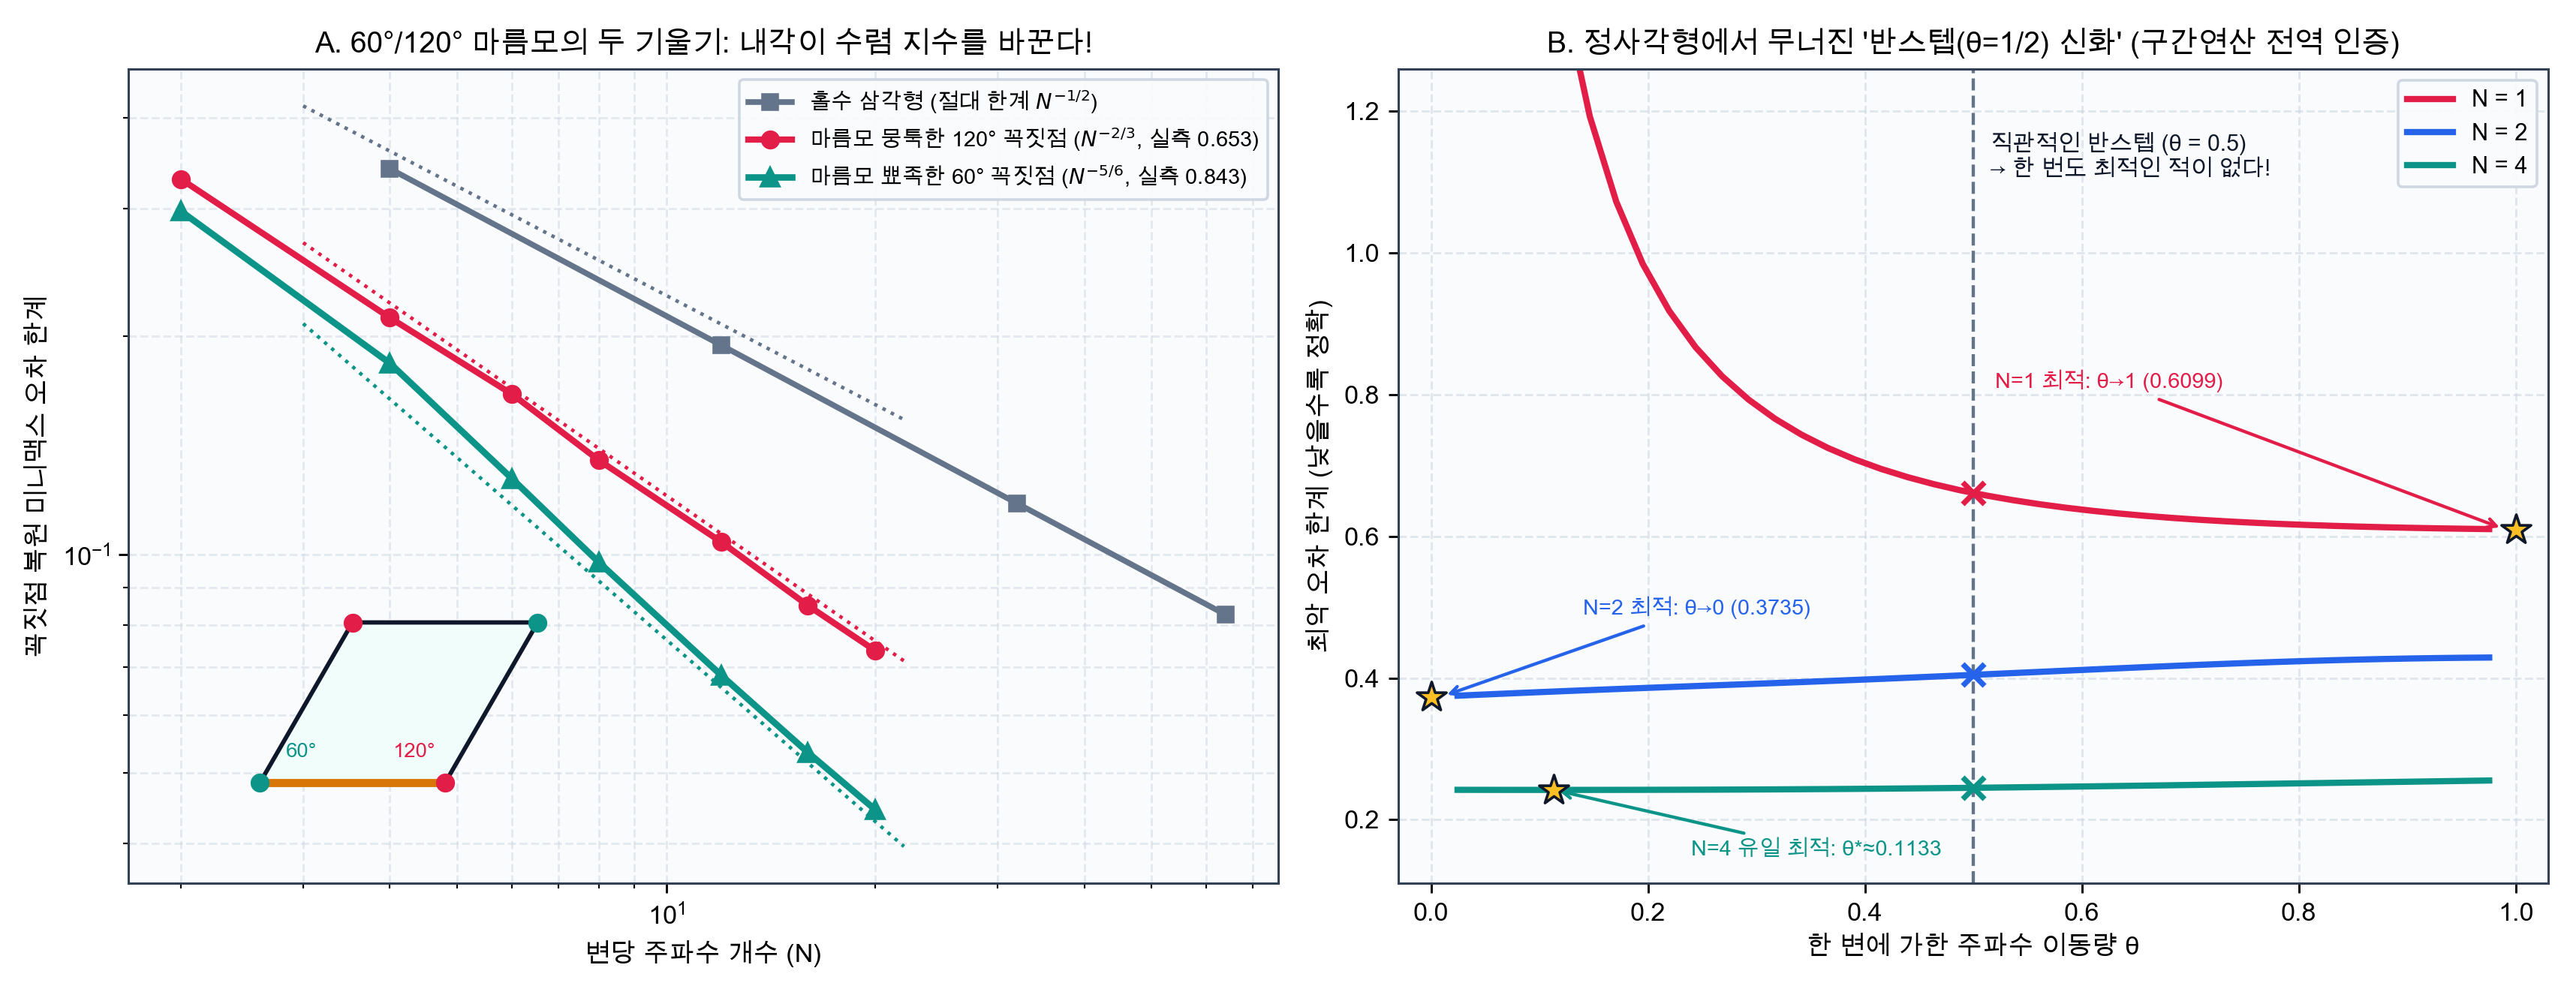
\includegraphics[width=\textwidth]{figs/kr_fig3_parity_and_rhombus.png}
\caption{\textbf{A.} $60^\circ/120^\circ$ 마름모 하나에서 동시에 나타나는 두 수렴 지수: $60^\circ$ 꼭짓점은 $N^{-5/6}$, $120^\circ$ 꼭짓점은 $N^{-2/3}$로 수렴하며 홀수 삼각형의 한계 $N^{-1/2}$를 돌파한다(28개 위험도 값 모두 45자리 일치). \textbf{B.} 단위 정사각형에서 구간연산으로 인증한 `반스텝($\theta=1/2$) 신화'의 붕괴.}
\end{figure}

\begin{itemize}
  \item \textbf{[기적 4] 홀짝 은폐 역설과 단일 이동 해독}: 홀수 다각형은 이웃 합 $a_j+a_{j+1}$만으로 모든 전하가 풀리지만, 모든 짝수 다각형에서는 교대 전하 $(+1,-1,+1,-1)$가 평균 극한에서 $0$으로 소거된다(특히 정사각형·평행사변형에서는 모든 정수 주파수에서 정확히 $0$이 된다!). 그러나 \textbf{단 한 변}의 주파수를 $(m-1+\theta)b_1$로 이동하면 극한이 $a_1 + e^{2\pi i\theta}a_2$로 바뀌어 즉시 해독된다(정사각형 $\theta=1/2$ 첫 샘플에서 $2(1-e^{-\pi}) = 1.91357216$ 검출). 단, 이동 샘플을 딱 1개만 추가할 때는 고정 주파수나 대역 끝($m=N-1$)에 두면 영구 오차 바닥이 남고, 대역 내부(예: 비례 내부 위치)에 두어야 $O(N^{-1/2})$ 수렴이 살아난다.
  \item \textbf{[기적 5] 각도가 수렴 지수를 바꾼다 ($60^\circ/120^\circ$ 마름모 실험)}: 배경 한계 $\|g\|_{L^2}\le M$ 아래 모든 선형·비선형 추정기를 통틀어, 홀수 다각형의 미니맥스 오차는 절대 \textbf{$N^{-1/2}$}을 넘지 못한다(지정된 부등변 삼각형 꼭짓점에서는 보정 평균이 최적 선형 추정기보다 $27\%$ 이상 비효율적임도 확인됐다). 그런데 짝수 다각형의 한 변에 $N$개의 이동 주파수를 추가하면 \textbf{$N^{-1/2}$ 장벽이 깨지며 꼭짓점 내각 $\omega_k$가 수렴 지수를 결정한다!}
  \begin{equation}
    E_k(N) \asymp_D M \cdot N^{-(1 - \omega_k/(2\pi))}.
  \end{equation}
  실제로 $60^\circ$와 $120^\circ$ 내각을 함께 가진 마름모에서 100자리·132자리 계산(28개 위험도 전부 유효숫자 45자리 일치)을 수행한 결과, \textbf{뾰족한 $60^\circ$ 꼭짓점은 $N^{-5/6}$}(실측 $0.843$), \textbf{뭉툭한 $120^\circ$ 꼭짓점은 $N^{-2/3}$}(실측 $0.653$)로 동시에 갈라졌다!
  \item \textbf{[기적 6] `반스텝($\theta=1/2$) 신화'의 붕괴}: 230자리 외향 반올림 구간연산으로 단위 정사각형의 전역 위험도를 검증한 결과, 직관적인 반스텝 $\theta=1/2$은 $N=1,2,4$ 어디에서도 최적이 아니었다! $N=1$은 $\theta\uparrow 1$ 극한(기존 샘플과 충돌하며 복소 미분 $B'(b_1)$ 정보 획득), $N=2$는 $\theta\downarrow 0$ 극한(원점으로 다가가며 총질량과 방향 모멘트 획득)에서 최소가 되고, $N=4$는 $\theta^* \approx 0.113299$에서 유일한 내부 최솟값을 갖는다.
\end{itemize}

\section{기적 7: 24자릿수 초해상도, 포카스 PDE 완치, 가열 금속판과 기계 증명}

\begin{itemize}
  \item \textbf{약 24자릿수(23.5 orders) 초해상도 윈도우}: 배경 플럭스가 매끄러울 때 일반 보정 평균은 $1/m$ 경계항 때문에 $N=128$에서도 오차가 삼각형 $1.9\times 10^{-2}$, 정사각형 $2.5\times 10^{-2}$에 머문다. 반면 역거듭제곱 $x_m^{-1},\dots,x_m^{-r}$을 대수적으로 소거하는 $8$차 외삽 가중치 $w_i = \frac{(-1)^{r-i} x_i^r}{d^r i!(r-i)!}$를 적용하면 오차가 \textbf{삼각형 $6.0\times 10^{-26}$, 정사각형 $8.3\times 10^{-26}$으로 약 23.5자릿수 급감}한다!(체비쇼프 증폭 하한 $\|w\|_1 \ge |T_r(\frac{a+b}{b-a})|$ 동시 규명.)
  \item \textbf{포카스 PDE 영공간 완치 \& 가열 금속판}: 무한 정수 격자 콜로케이션의 정확한 $2k-1$차원 영공간 정리를 바탕으로, 조각별 일차함수+투명 기저 시험 공간(변당 5모드)에 저차 모멘트 $2k-1$개를 보완해 조건수를 $16.45$(사각형), $12.21$(삼각형)로 낮추고 내부 조화장을 \textbf{$3.9\times 10^{-16}$} 정밀도로 복원했다. 또한 벽 온도가 불연속($1^\circ\text{C}, 4^\circ\text{C}, -2^\circ\text{C}, 5^\circ\text{C}$)인 금속판의 발산 열유속이 정칙 시험함수에 대한 양측 유한부분(Hadamard finite part) 아래 $B_{\mathrm{fp}\,q_n}(s) = i\sum a_j e^{s\gamma_j}$를 만족함을 $7.1\times 10^{-14}$ 정밀도로 검증했다.
  \item \textbf{Lean~4.36.0 기계 검증}: 홀짝 순환 역설과 단일 이동 해독, 유한 차원 비선형 미니맥스 하한 대수, 유리수 외삽 윈도우의 역거듭제곱 소거 항등식, 유리수 양방향 대칭 붕괴 및 방데르몽드 그룹화 등 \textbf{핵심 대수 기둥 31개 정리를 순수 Lean~4 코드(\texttt{sorry} 0개)로 형식 검증}했다.
\end{itemize}

\begin{figure}[ht]
\centering
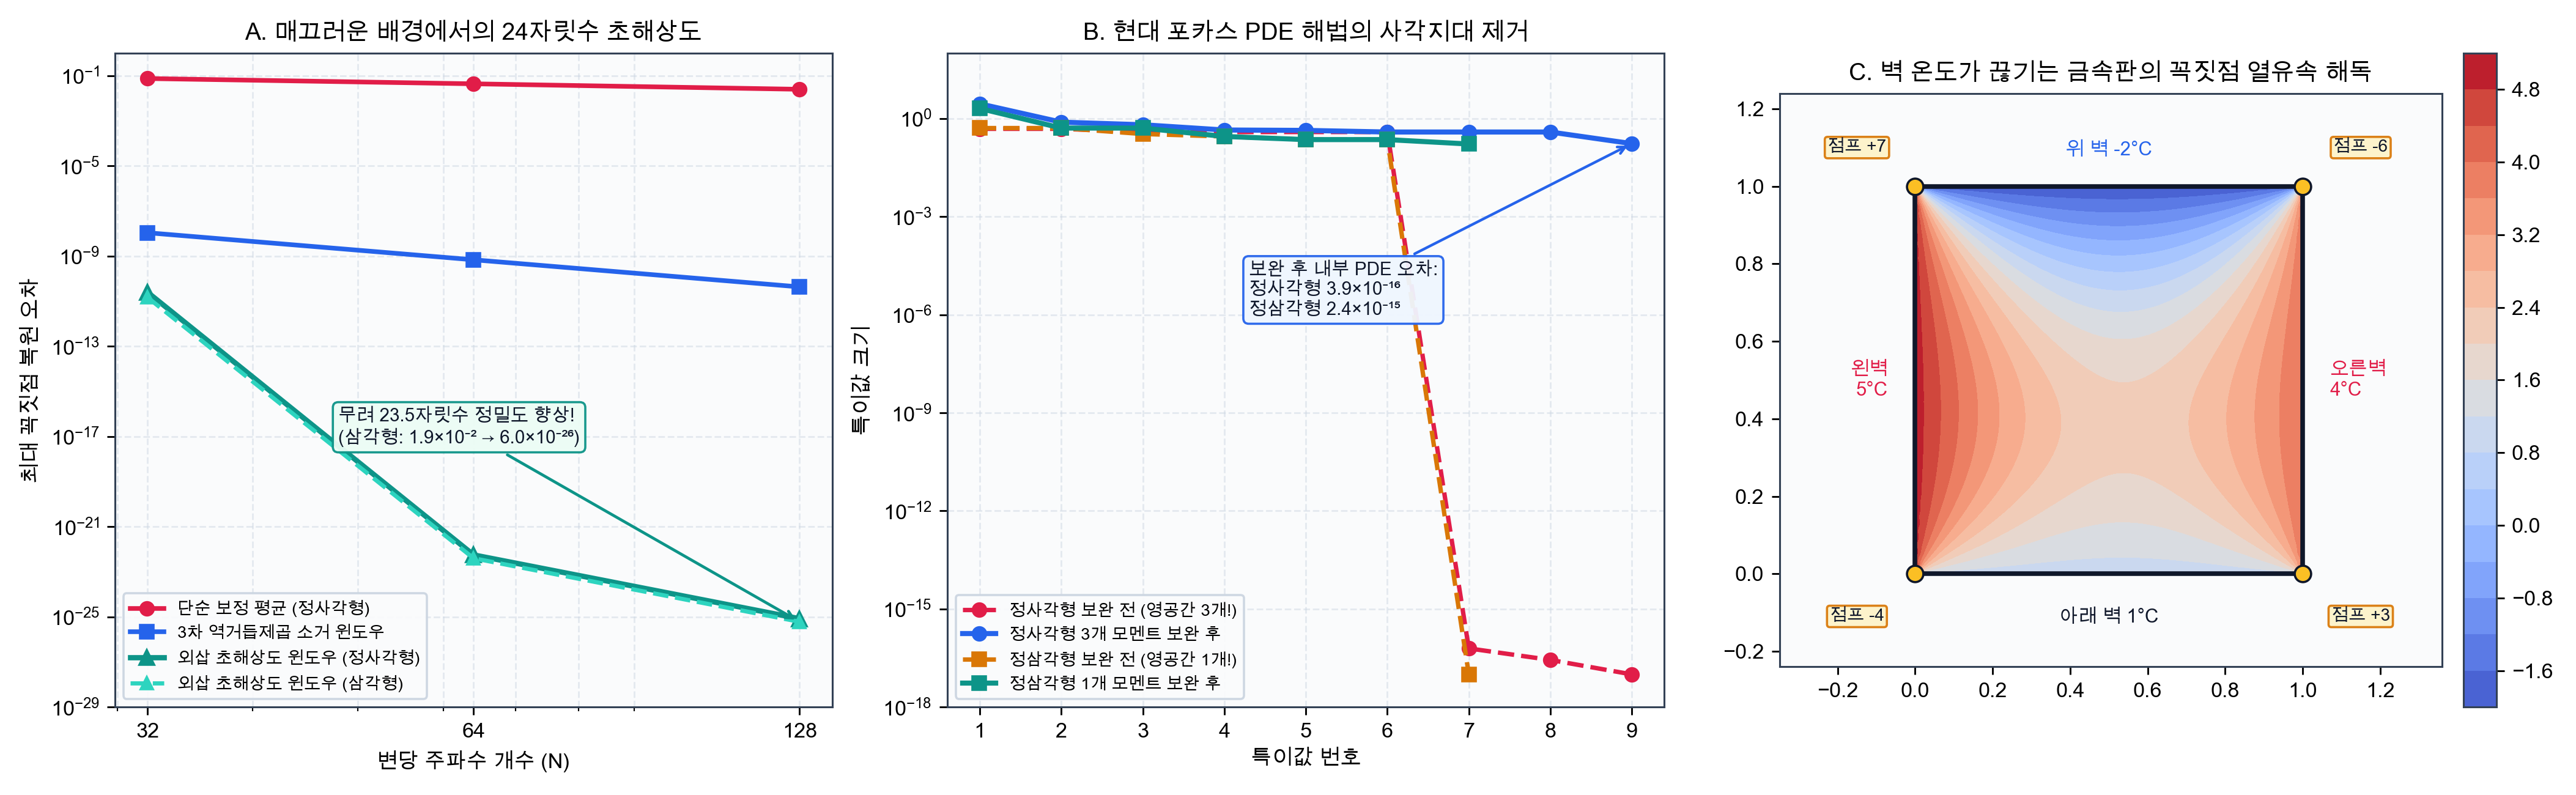
\includegraphics[width=\textwidth]{figs/kr_fig4_superres_and_plate.png}
\caption{\textbf{A.} 역거듭제곱 소거 윈도우를 통한 초해상도 복원. \textbf{B.} 모멘트 보완 전후의 포카스 PDE 특이값 스펙트럼($\kappa=16.45, 12.21$). \textbf{C.} 벽 온도가 끊기는 금속판의 온도장과 꼭짓점 점프 해독.}
\end{figure}

50년 전 우랄 산맥 너머에서 종이와 펜만으로 지수급수의 지도를 그렸던 한 소련 수학자의 유산은 결코 낡은 유물이 아니었다. 현대 편미분방정식, 확률론, 초해상도 역문제, 그리고 기계 검증이라는 새로운 렌즈를 들이대자마자, 잊혔던 기하학적 세계가 지금 다시 살아 움직이고 있다.

\end{document}
